\title{Implementing a Multithreading Library}
\author{
        Louis Cameron Booth \\
                louiscb@kth.se\\
                9704181917
                \\
                \\
}
\date{\today}

\documentclass[11pt]{article}
\usepackage{pgfplots}
\usepackage{graphicx}
\usepackage[font=small,labelfont=bf]{caption}
\captionsetup[figure]{position=above}

\begin{document}
\maketitle

\pagebreak
\section{Introduction}
In this report we will discuss the POSIX Threads API. We will develop our own simplified versions of the core functions from the API's implementation in the C standard library \textit{pthread}. We will then compare the performance of the pthread library to our own library which have called \textit{green}. 

\section{Multithreading}\label{Multithreading}

The POSIX thread library is an API for spawning and handling multiple threads. Each thread of a multithreaded program can be viewed as its own independent entity, except for the fact that they share data and the same address space. It is used to achieve parallelisation, where a single process can perform work simultaneously on a machine. A normal program will have a single point of execution, whilst a program that utilises the pthread library can have multiple points of execution. 

The pthread library contains dozens of POSIX thread functions that allow multiple flows of control for an eligible program. However in this report we only focus on a few of the fundamental functions that form the core of building a multithreaded program.

Multithreaded programs make use of execution contexts. An execution context is the information relating to the task's current execution state and may consist of a heap, stack, code, instruction pointer and processor registers. The use of an execution context in \textit{this} context is that we can store a program's state in the computer's memory and then return to the same place we were by moving the context back to the CPU's registers. This is useful for multithreading as it permits us to interrupt a thread, save its context, run another thread, and then return to the original thread right where we left off.

\section{Our Implementation}

You can view all of our code and run the program by downloading the directory at: \underline{www.github.com/louiscb/Operating-Systems/tree/master/threads/green}
\\
\\
Our thread library is called green and contains the main functions necessary to create a multithreaded program.

At the very core of our implementation, and the key concept to understanding the code, is a humble queue. The queue contains a list of threads ready to be executed, and is aptly named \textit{readyQueue}. The thread management system chooses the thread to be executed by dequeuing from readyQueue and then running that thread's context (see figure 1). The only way a thread is ever run is by it joining the back of the queue and waiting for its turn at the front. There are several situations where a thread can be enqueued or dequeued from the readyQueue, and we will go into more detail with that later.

\includegraphics[width=12cm]{queueDiagram}
\captionof{figure}{Our queue for ready threads}

As just mentioned, we make use and rely on the concept of an execution context in order to permit multithreading. We utilise the C library \textit{ucontext} to save and switch between our thread's contexts.

In total we have nine functions in our library's API that are related to thread management and we will go through each of them.

\subsection{Create a thread: \textit{green\_create}}

This function initialises the thread and allocates it space on the heap. We use our own struct \textit{green\_t} which contains pointers to that thread's context, as well as a few other pieces of data. It is our equivalent of the pthread library's \textit{pthread\_t}.

\subsection{Yield a thread: \textit{green\_yield}}

This function suspends the current running thread and selects a new thread for execution. It is our version of pthread\_yield. The function puts the running thread last in the ready queue and then selects the first thread from the queue as the next thread to run.
\subsection{Wait for a thread termination: \textit{green\_join}}

The current thread will be suspended until a chosen thread has finished executing. This is used so that a main thread doesn't return before a child thread has finished processing. This is our version of pthread\_join.

\subsection{Initialise a condition variable: \textit{green\_cond\_init}}

This function creates a condition variable. Condition variables are useful when communication between threads is necessary, for example if one thread needs another to do something before it can continue. Equivalent to pthread\_cond\_init.

\subsection{Suspend the current thread: \textit{green\_cond\_wait}}

We suspend the current thread on our condition variable. What this means is that we put the calling thread to sleep, and it remains like this until another thread signals it to wake up. Equivalent to pthread\_cond\_wait.

\subsection{Unblock a suspended thread: \textit{green\_cond\_signal}}

Moves a suspended thread to the ready queue to be executed. This is called after a thread has completed an action that another thread would be waiting for. Equivalent to pthread\_cond\_signal.

\subsection{Initialise a mutex: \textit{green\_mutex\_init}}

Create a mutex lock used to protect critical sections of a program. Equivalent to pthread\_mutex\_signal.

\subsection{Lock a mutex: \textit{green\_mutex\_lock}}

This is called when you have a region of code that needs to be protected to ensure that only one thread is running it at a time. If no other thread holds the lock when this function is called, this thread will take the lock until it unlocks it. However, if the lock is already taken, the thread will remain in this function and will only return once the lock has become free and it can take it. Equivalent to pthread\_mutex\_lock.

\subsection{Unlock a mutex: \textit{green\_cond\_unlock}}

Used when you are done with a critical section and wish to free the lock. Equivalent to pthread\_mutex\_unlock.

\subsection{Timers}

We make use of timers in our library to perform interrupts at regular intervals for running threads. When a timer interrupt occurs, the current thread is suspended and the next thread is taken from the ready queue. An issue that arose with this method is that the interrupts might occur whilst the program was in the middle of a thread management function, and not a thread function. This would result in the management of threads being interrupted, which could corrupt the entire multithreading process. Our solution was to create two functions, \textit{blockTimer, unblockTimer}, which would be called at the beginning and end of a thread's function which meant that the timers would only be allowed to interrupt during the running of a thread. 
\\
\\
The example below shows a test function that utilises timers and mutexes. The overall change to the global counter variable should be 0. However without the mutex calls, multiple running threads would interrupt each other before the counter value was decreased and the value of counter would be unpredictable.

\begin{verbatim}
void *test(void *arg) {
    unblockTimer();
    
    green_mutex_lock(&mutex);
    counter+=1;

    //spin to slow down function, interrupt probably occurs here
    for (int c = 1; c <= 3270; c++)
        for (int d = 1; d <= 3270; d++)
        {}

    counter-=1;
    green_mutex_unlock(&mutex);
    blockTimer()
}
\end{verbatim}

\section{Testing}\label{Testing}

In order to draw comparisons between our green thread library and the pthread library we have performed some benchmark tests. 

\subsection{Method}

We evaluated the different libraries by measuring the time taken to return from specific functions. Both libraries used identical functions, and we increased the number of threads that executed these functions in order to see a change in execution time. We used the clock() method included in the time.h library and we measured the difference between the time before and after calling our functions.

\subsection{Results}

We ran tests on the yield, condition, mutex, and timer functionalities we implemented in our green library.
\\
\\
To test our yield method, we spawned n number of threads and assigned each thread a function that decremented a local variable 1000 times. At the end of each decrement the thread yielded. We ran this test for both libraries and inputted a large number of threads: from 10 to 50,000. In Figure 2 you can the plotted results of that test. 
\\
\\
The rest of the functions provided much less interesting, and perhaps alarming, data. We wrote equivalent testing functions using condition variables, timers and mutexes as we did for the yield functions. Our library kept up with the pthread library, with both libraries taking 0ms to run every permutation. This was until we approached 100 threads, at this point our thread library began breaking and displaying segmentation errors. 

\resizebox {\columnwidth} {!} {
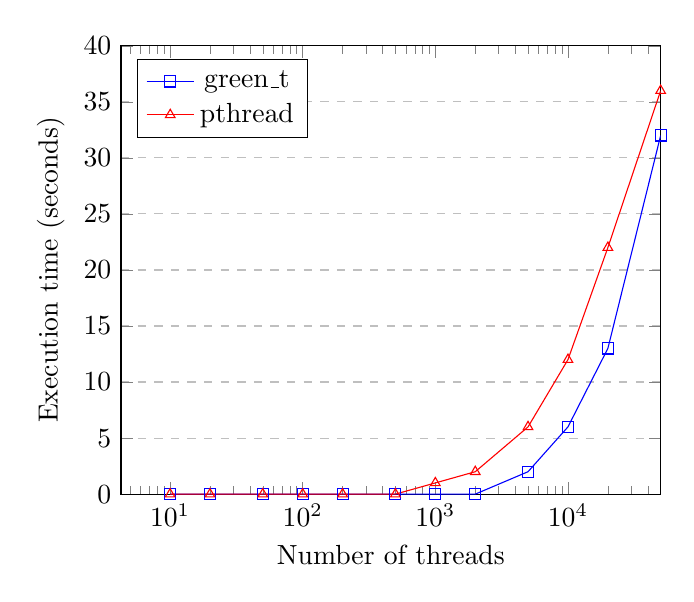
\begin{tikzpicture}
\begin{axis}[
    xmode=log,
    xlabel={Number of threads},
    ylabel={Execution time (seconds)},
    xmin=0, xmax=50000,
    ymin=0, ymax=40,
    ytick={0,5,10,15,20,25,30,35,40},
    legend pos=north west,
    ymajorgrids=true,
    grid style=dashed,
]
\addplot[
    color=blue,
    mark=square,
    ]
    coordinates {
    (10,0)(20,0)(50,0)(100,0)(200,0)(500,0)(1000,0)(2000,0)
    (5000,2)(10000,6)(20000,13)(50000,32)
    };
     \addlegendentry{green\_t}
\addplot[
    color=red,
    mark=triangle,
    ]
    coordinates {
    (10,0)(20,0)(50,0)(100,0)(200,0)(500,0)(1000,1)(2000,2)
    (5000,6)(10000,12)(20000,22)(50000,36)
    };
    \addlegendentry{pthread}
\end{axis}
\end{tikzpicture}
}
\captionof{figure}{Execution time of yield green\_t vs pthread}

\subsection{Analysis}

The above results show that our implementation was faster than pthread for a  yield function. We believe this occurs because this is an extremely simple and straightforward test with only one call to a thread API in the thread's function. The green library is very lightweight and in this situation there are much fewer overheads in comparison to pthread, which has more of an emphasis on error catching and quality control. When it comes to the more complicated tests, such as the condition variables test, there is much more going on. With this test there are now four calls to the thread API in every thread's function, we are using timers and multiple queues. Once we get to 100+ threads the rawness and inefficiencies of the green library are made more apparent and this is where our library breaks down.

\section{Conclusions}\label{conclusions}

The POSIX API is a library that has become a core of modern computer systems. All  operating systems worth their salt perform software multithreading and it is vital that the management of these threads occurs without a hitch, after all a single misbehaving thread can crash the entire process it lives within. Multithreading is something that should occur so smoothly under the hood that higher-level programmers and general users shouldn't even know it exists. 
Although our green library permits you to create and manage threads and perform a wide variety of management techniques, I don't think I would trust as the basis of an air traffic control operating system.

\end{document}
This is never printed



















